\documentclass[journal]{IEEEtran}

% Packages
\usepackage{cite}
\usepackage{graphicx}
\usepackage{subfigure}
\usepackage{float}
\usepackage{url}
\usepackage{color}

\sloppy
\definecolor{lightgray}{gray}{0.5}

\begin{document}

% paper title
% can use linebreaks \\ within to get better formatting as desired
\title{Autonomous Robotics Lab 1 \\ Brushfire and Wavefront}
%
%
% author names and IEEE memberships
% note positions of commas and nonbreaking spaces ( ~ ) LaTeX will not break
% a structure at a ~ so this keeps an author's name from being broken across
% two lines.
\author{Rodrigo Caye Daudt}





% make the title area
\maketitle




% Note that keywords are not normally used for peerreview papers.
%\begin{IEEEkeywords}
%IEEEtran, journal, \LaTeX, paper, template. ln505
%\end{IEEEkeywords}



%%%%%%%%%%%%%%%%%%%%%%%%%%%%%%%%%%%%%%%%%%%%%%%%%%%%%%%%%%%%%%%%%%%%%%%%%%%%%%%
\section{Introduction}

\IEEEPARstart{T}{his} report describes implementations in MATLAB for the Brushfire and Wavefront algorithms developed for the Autonomous Robotics module. These algorithms are used for path planning based on a given map. Sections \ref{brushfire} and \ref{wavefront} describe the implementations and results of the Brushfire and Wavefront algorithms, respectively, Section \ref{discussion} contains an analysis of the obtained results, and Section \ref{conclusion} concludes this work.

%%%%%%%%%%%%%%%%%%%%%%%%%%%%%%%%%%%%%%%%%%%%%%%%%%%%%%%%%%%%%%%%%%%%%%%%%%%%%%%
\section{Brushfire}\label{brushfire}

The Brushfire algorithm serves to create a potential function that guides a robot away from the obstacles. Starting from the walls and objects, which are initialised with value 1, the algorithm spreads from these starting points (in this case using 8-neighbourhood) in generations until all of the map has been covered. In other words, the Brushfire algorithm calculates the small 8-neighbourhood distance to an obstacle for every point in the map. A parallel can be made to the way fire spreads in the real world. It is important to note that this algorithm assign high values to points distant to obstacles, not low values.

The Brushfire algorithm was implemented to work in generations of points. Instead of keeping one single queue of points to be analysed next, the function keeps two queues: one for the points in the current generation (all of which have the same distance from obstacles), and one for the points that were added during the current generation and that will be processed on the next batch. This procedure leads to a resizing of smaller MATLAB arrays, which is faster since it requires smaller memory allocations. The algorithm stops when a generation ends and the list of points to be processed is empty. The code for \textit{brushfire.m} can be found in Appendix \ref{brushm}.

Figures \ref{basic_bf}-\ref{obstaclesBig_bf} contain the results of the Brushfire algorithm over the four provided maps displayed using a jet colour map (low values in blue, high values in dark red). It can be observed that the walls and obstacles are displayed in blue and the temperature of the color increases as the distance from the walls and object increases, which was expected since the smallest labels (1) are assigned to the fixed objects and progressively larger are assigned to points farther from these objects. The computational times will be discussed in section \ref{discussion}.


\begin{figure}\label{basic_bf}
	\centering
	
\includegraphics[width=0.8\linewidth]{figures/basic_bf.png}
	\caption{Brushfire - basic.mat}
\end{figure}

\begin{figure}\label{maze_bf}
	\centering
	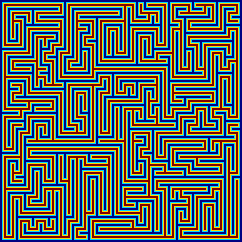
\includegraphics[width=0.8\linewidth]{figures/maze_bf.png}
	\caption{Brushfire - maze.mat}
\end{figure}

\begin{figure}\label{mazeBig_bf}
	\centering
	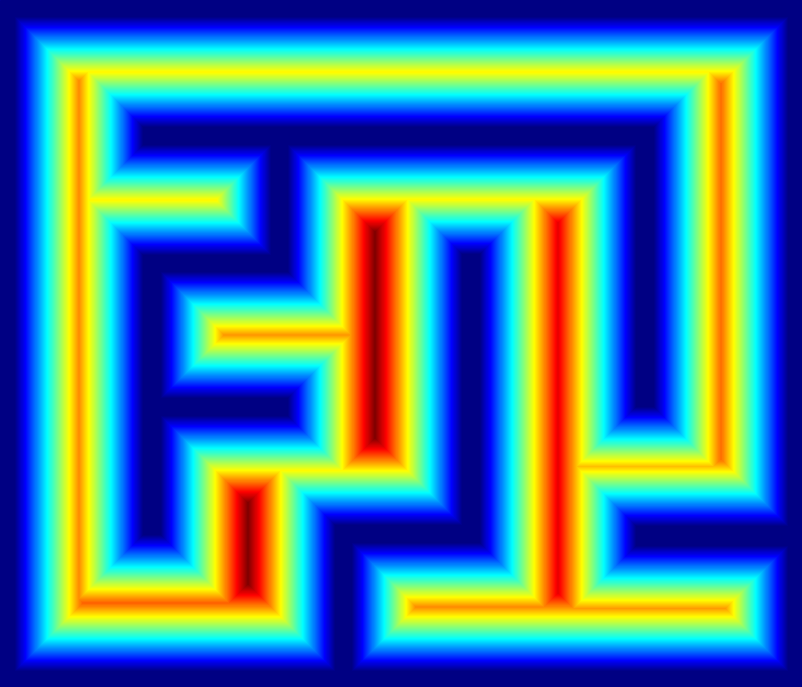
\includegraphics[width=0.8\linewidth]{figures/mazeBig_bf.png}
	\caption{Brushfire - mazeBig.mat}
\end{figure}

\begin{figure}\label{obstaclesBig_bf}
	\centering
	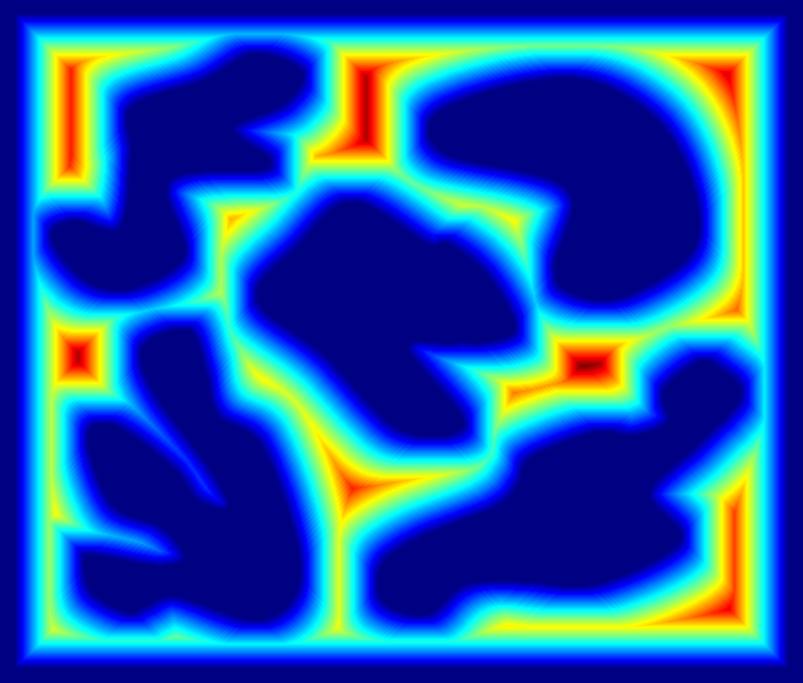
\includegraphics[width=0.8\linewidth]{figures/obstaclesBig_bf.png}
	\caption{Brushfire - obstaclesBig.mat}
\end{figure}



%%%%%%%%%%%%%%%%%%%%%%%%%%%%%%%%%%%%%%%%%%%%%%%%%%%%%%%%%%%%%%%%%%%%%%%%%%%%%%%
\section{Wavefront}\label{wavefront}

The Wavefront algorithm's purpose is to find a path from a given starting point in the map to a given goal. It works in a similar way to the Brushfire algorithm, but instead of expanding from the walls and obstacles, it starts from the goal point and expands using the 8-neighbourhood of each pixel until it reaches every point in the map. It is important to notice that even though the starting point is not part of an obstacle, the waves cannot pass through the fixed objects defined in the map.

Given the similarities between the Wavefront and the Brushfire algorithms, their implementations were very similar. That means the Wavefront was implemented using the same generational principle and for the same reasons as described in Section \ref{brushfire}.

It was also required to use the \textit{wavefront} function to calculate one of the possible good paths from the chosen starting point to the goal point. This was made by creating a sequential list of points where each point had an associated value smaller by 1 relative to the previous entry. Priority was given to the cross-neighbours (4-neighbourhood), since they yield a smaller distance than the diagonal neighbours. This was done by checking the cross-neighbours before the diagonals, and picking the first point with an associated wavefront value smaller than the current value. The code for \textit{wavefront.m} can be found in Appendix \ref{wavem}.

Figures \ref{basic_wf}-\ref{obstaclesBig_wf} show the results of the \textit{wavefront} function over the four provided maps, with an overlaid trajectory for example starting points and goals. The maps are displayed with a parula colour map (blue for low values, yellow for high values), the calculated trajectory is displayed in red, a black dot marks the starting point and a yellow dot marks the goal. We can see this algorithm allows us to find a smart trajectory from the starting points to the goals as long as the two points can be connected. This algorithm is very robust and works in any type of environment, independently of the shapes of the objects in the map. It can also be observed that horizontal and vertical directions are prioritized, and diagonal directions are chosen only when the Carthesian directions don't provide any steps that decrease the distance to the goal.

\begin{figure}\label{basic_wf}
	\centering
	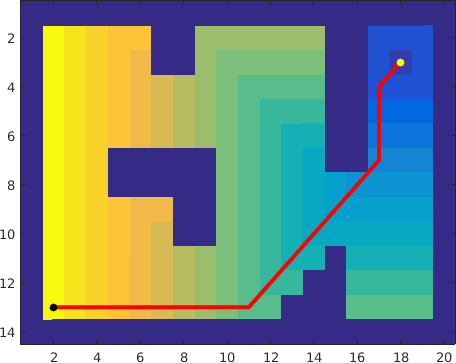
\includegraphics[width=0.8\linewidth]{figures/basic_wf.png}
	\caption{Wavefront - basic.mat}
\end{figure}

\begin{figure}\label{maze_wf}
	\centering
	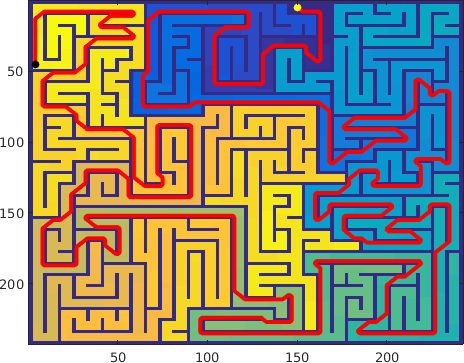
\includegraphics[width=0.8\linewidth]{figures/maze_wf.png}
	\caption{Wavefront - maze.mat}
\end{figure}

\begin{figure}\label{mazeBig_wf}
	\centering
	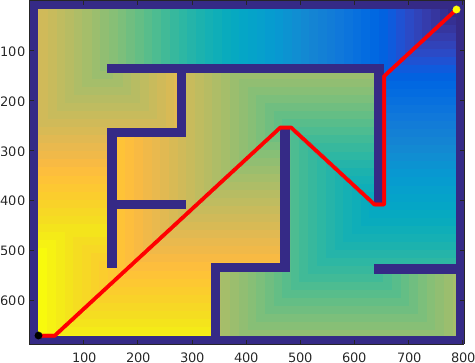
\includegraphics[width=0.8\linewidth]{figures/mazeBig_wf.png}
	\caption{Wavefront - mazeBig.mat}
\end{figure}

\begin{figure}\label{obstaclesBig_wf}
	\centering
	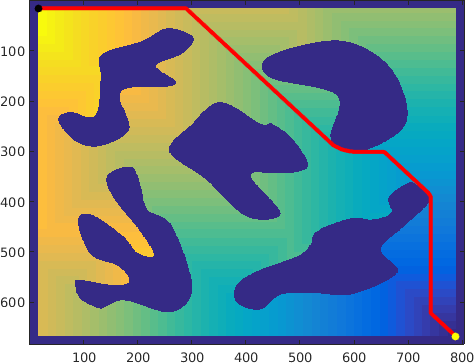
\includegraphics[width=0.8\linewidth]{figures/obstaclesBig_wf.png}
	\caption{Wavefront - obstaclesBig.mat}
\end{figure}



%%%%%%%%%%%%%%%%%%%%%%%%%%%%%%%%%%%%%%%%%%%%%%%%%%%%%%%%%%%%%%%%%%%%%%%%%%%%%%%
\section{Discussion}\label{discussion}

From the results shown in Sections \ref{brushfire} and \ref{wavefront} we can observe that both algorithms are very stable. The Brushfire algorithm can be calculated for all points in the map, while the Wavefront algorithm can be calculated for all points that can be connected to the goal, and, if possible, a trajectory between the starting point and the goal will be found. Together, these algorithms are very powerful for path planning of mobile robots.

One disadvantage of these algorithms is that they assume that the map is completely known, which in only true for a limited range of real world applications. The usage of these algorithms with maps that are updated in real time (using SLAM for example) would require frequent recalculation of the potential maps and trajectories, and it could be very demanding or impossible for a simple microprocessor to do it in real time for medium and large maps.

The table in Fig. \ref{times} shows the calculation times for the application of the Brushfire and the Wavefront algorithms to the four provided maps. These times were obtained using MATLAB running on one core of an Intel$^R$ Core$^{TM}$ i7-5500U CPU @ 2.40GHz. It is important to point out that even when running on a strong modern processor the computing times for large maps are not fit for real time applications if it is recomputed at every cycle.


\begin{figure}[H]\label{times}
\centering
\begin{tabular}{l | r r r}
Map & Num. of pixels & Brushfire & Wavefront \\
\hline
basic.m & 280 & 0.013045 & 0.007583 \\
maze.m & 58564 & 0.786043 & 0.169837 \\
mazeBig.m & 550974 & 4.674438 & 1.861244 \\
obstaclesBig.m & 548449 & 4.005892 & 1.345025 \\
\end{tabular}
\caption{Execution times, in seconds, of the Brushfire and Wavefront algorithms over the four provided maps}
\end{figure}


%%%%%%%%%%%%%%%%%%%%%%%%%%%%%%%%%%%%%%%%%%%%%%%%%%%%%%%%%%%%%%%%%%%%%%%%%%%%%%%
\section{Conclusion}\label{conclusion}

We described and analysed implementations of the Brushfire and the Wavefront algorithms. Both algorithms proved to be very robust, but may not be fit for real time recalculations. 

We also observed that the Wavefront algorithm prioritizes a minimum distance to the goal in the computed trajectory, while the Brushfire algorithm is not affected by starting points or goals, since it only guides a robot to stay away from obstacles. This indicates that these two algorithms could be used in conjunction to calculate a trajectory which may not me the shortest possible, but balances between distance and safety by staying far from the obstacles throughout the trajectory.




\appendices


\begin{figure*}
\section{brushfire.m}\label{brushm}
    \begin{verbatim}
function [value_map] = brushfire(map)
% Brushfire algorithm for repulsive potential
% Rodrigo Daudt

    % Initialise value_map
    value_map = map;

    % Find initial values
    s = size(map);
    initials = find(map==1);
    [queue(:,1) queue(:,2)] = ind2sub(s,initials);

    % Offsets for neighbours
    N = [1 0;-1 0;0 1;0 -1;1 1;1 -1;-1 1;-1 -1];

    cl = 2; % Current label
    next_queue = [];

    while size(queue,1) > 0
        for i = 1:size(queue,1)
            for neigh = 1:size(N,1)
                v = queue(i,1) + N(neigh,1);
                h = queue(i,2) + N(neigh,2);
                if v>=1 && v<= s(1) && h>=1 && h<=s(2)
                    if value_map(v,h)==0
                        value_map(v,h) = cl;
                        next_queue = [next_queue;v h];
                    end
                end
            end
        end
        cl = cl + 1;
        queue = next_queue;
        next_queue = [];
    end
end
\end{verbatim}
\color{black}
\end{figure*}




\begin{figure*}
\section{wavefront.m}\label{wavem}
    \begin{verbatim}
function [value_map, trajectory] = wavefront(map, start, goal)
% Wavefront path planning
% Rodrigo Daudt

    % Initialise value_map
    value_map = map;
    value_map(goal(1),goal(2)) = 2;

    % Find map size
    s = size(map);

    % Offsets for neighbours
    N = [1 0;-1 0;0 1;0 -1;1 1;1 -1;-1 1;-1 -1];

    cl = 3; % Current label
    queue = [goal(1) goal(2)]; % Current level queue
    next_queue = []; % Next level queue

    while size(queue,1) > 0
        for i = 1:size(queue,1)
            for neigh = 1:size(N,1)
                v = queue(i,1) + N(neigh,1);
                h = queue(i,2) + N(neigh,2);
                if v>=1 && v<= s(1) && h>=1 && h<=s(2)
                    if value_map(v,h)==0
                        value_map(v,h) = cl;
                        next_queue = [next_queue;v h];
                    end
                end
            end
        end
        cl = cl + 1;
        queue = next_queue;
        next_queue = [];
    end

    % Find trajectory
    cp = start; % current point
    trajectory = [start(1) start(2)];

    while value_map(cp(1),cp(2)) ~= 2
        for i = 1:size(N,1)
            % Neighbour coordinates
            v = cp(1) + N(i,1);
            h = cp(2) + N(i,2);
            if v>=1 && v<= s(1) && h>=1 && h<=s(2)
                if value_map(v,h) == (value_map(cp(1),cp(2))-1)
                    cp = [v h];
                    trajectory = [trajectory;cp];
                    break;
                end
            end
        end
    end
end
\end{verbatim}
\end{figure*}


% use section* for acknowledgement
%\section*{Acknowledgment}
%The authors would like to thank...


%\bibliographystyle{IEEEtran}
%\bibliography{Template_Daudt}


\end{document}


